\chapter{Využití vodíku jako nosiče energie}

I přesto, že se vodík v průběhu let ukázal jako možný klíčový nosič energie kvůli jeho možnosti sloužit jako dekarbonizační prostředek, je jeho dosavadní využití soustředěné pouze na určitá odvětví strojního a chemického průmyslu. \cite{Griffiths2021,IEAfuture} Na Obr. \ref{fig:pouziti_vodiku_proc} je vyjádřené procentuální vyjádření celosvětové poptávky po vodíku od roku $2000$ pro dané použití v čisté formě, kde je dovolené pouze malé množství aditiv nebo nečistot, a v sloučeninách, například syntézního plynu, který lze dále použít jako palivo nebo surovinu pro další procesy. \cite{IEAfuture}
\begin{figure}[h]
    \centering
    \definecolor{refining_pv}{RGB}{209,73,75}
\definecolor{ammonia_pv}{RGB}{252,186,29}
\definecolor{otherpure_pv}{RGB}{109,204,220}
\definecolor{methanol_pv}{RGB}{94,71,128}
\definecolor{dri_pv}{RGB}{168,149,196}
\definecolor{othermixed_pv}{RGB}{203,203,203}

\makeatletter
\newcommand\resetstackedplots{
\makeatletter
\pgfplots@stacked@isfirstplottrue
\makeatother
\addplot [forget plot,draw=none] coordinates{(2000,0) (2005,0) (2010,0) (2015,0) (2018,0)};
}
\makeatother

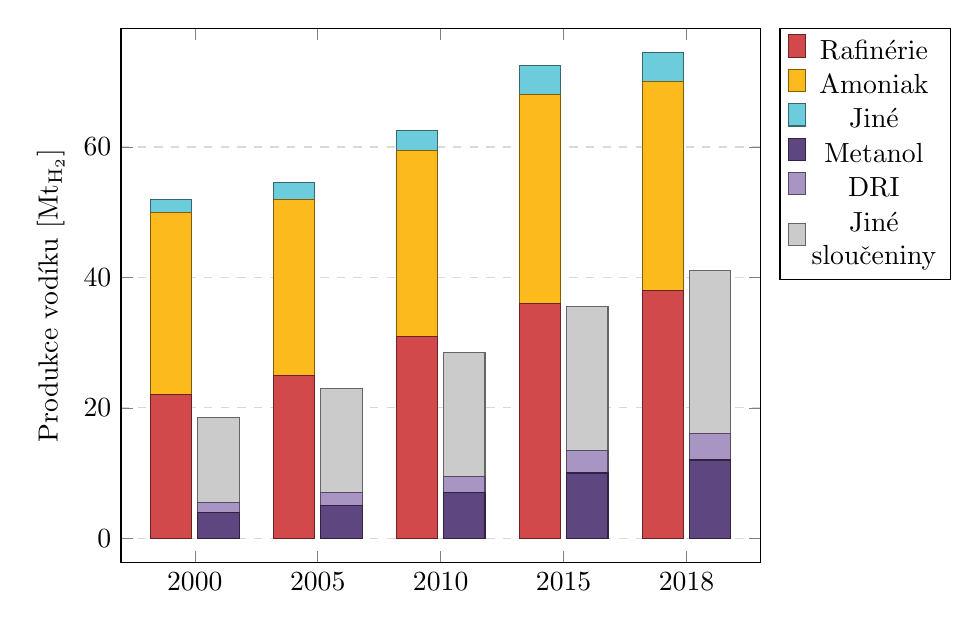
\begin{tikzpicture}
    \begin{axis}[
        ybar stacked,
        width = 0.8\textwidth,
        ymajorgrids,
        grid style={dashed,gray!30},
	bar width=15pt,
        enlarge x limits=0.15,
        enlarge y limits=0.05,
        ymin = 0,
        legend style={cells={align=center}},
        legend entries={Rafinérie,Amoniak,Jiné,Metanol,DRI,Jiné\\sloučeniny},
        legend pos=outer north east,
        ylabel={Produkce vodíku $[\mathrm{Mt_{H_2}}]$},
        symbolic x coords={2000,2005,2010,2015,2018},
        xtick=data,
    ]
        \addplot+[ybar,refining_pv!50!black,fill=refining_pv,text=black,bar shift=-.3cm] plot coordinates {(2000,22) (2005,25) (2010,31) (2015,36) (2018,38)};
        \addplot+[ybar,ammonia_pv!50!black,fill=ammonia_pv,text=black,bar shift=-.3cm] plot coordinates {(2000,28) (2005,27) (2010,28.5) (2015,32) (2018,32)};
        \addplot+[ybar,otherpure_pv!50!black,fill=otherpure_pv,text=black,bar shift=-.3cm] plot coordinates {(2000,2) (2005,2.5) (2010,3) (2015,4.5) (2018,4.5)};
        \resetstackedplots
        \addplot+[ybar,methanol_pv!50!black,fill=methanol_pv,text=black,bar shift=+.3cm] plot coordinates {(2000,4) (2005,5) (2010,7) (2015,10) (2018,12)};
        \addplot+[ybar,dri_pv!50!black,fill=dri_pv,text=black,bar shift=+.3cm] plot coordinates {(2000,1.5) (2005,2) (2010,2.5) (2015,3.5) (2018,4)};
        \addplot+[ybar,othermixed_pv!50!black,fill=othermixed_pv,text=black,bar shift=+.3cm] plot coordinates {(2000,13) (2005,16) (2010,19) (2015,22) (2018,25 )};
    \end{axis}
\end{tikzpicture}
    \caption[Celosvětová roční poptávka po vodíku podle využití od roku 2000]{Celosvětová roční poptávka po vodíku podle využití od roku 2000, převzato z \cite{IEAreview}.}
    \label{fig:pouziti_vodiku_proc}
\end{figure}

\section{Využití v chemickém průmyslu}
Většina vyrobeného vodíku se pak nejvíce používá jako reakční činidlo v chemickém, konkrétněji agrochemickém, nebo petrochemickém průmyslu. V těchto odvětvích se využívá tzv. syntézního plynu, který tvoří vodík společně s oxidem uhelnatým v daném stechiometrickém poměru. \cite{Seddon2022,IEAfuture}

\subsection{Výroba amoniaku}
Na výrobu amoniaku (\ce{NH3}) se ročně spotřebuje až 35$\%$ veškerého vyprodukovaného vodíku. Samotného amoniaku se ročně vyrobí a spotřebuje až $150\ \mathrm{Mt}$. Většina vyrobeného amoniak se dále zpracovává při výrobě hnojiv, nebo ho lze použít jako chladivo, popřípadě čistící činidlo. \cite{Seddon2022,Ramachandran1998}

Amoniak vzniká jako vedlejší produkt při pyrolýze uhlí, avšak většina čpavku je vyráběna synteticky. \cite{Chehade2021} Haberův–Boschův proces, který je v současnosti nejrozšířenějším procesem výroby amoniaku, je popsán následující exotermní reakcí
\reaction{3H2 + N2 -> 2NH3}
Při tomto procesu se syntézní plyn komprimuje na $\approx20\ \mathrm{MPa}$ a ohřívá na $\approx400\ \mathrm{^{\circ}C}$. Následně je přiveden do konventoru, kde za přítomnosti katalyzátoru (definice viz. \ref{subsec:premenytrp}) probíhá výše zmíněná reakce. Po ochlazení až na $-6\ \mathrm{^{\circ}C}$ amoniak zkondenzuje a nezkonvertovaný plyn se dále recykluje. Konečná konverze tohoto procesu se pohybuje kolem $12\ \mathrm{hm.}\%$. \cite{Seddon2022}
\begin{figure}[h]
    \centering
    \begin{tikzpicture}
\node[inner sep=0pt] (obrazek) at (0,0)
    {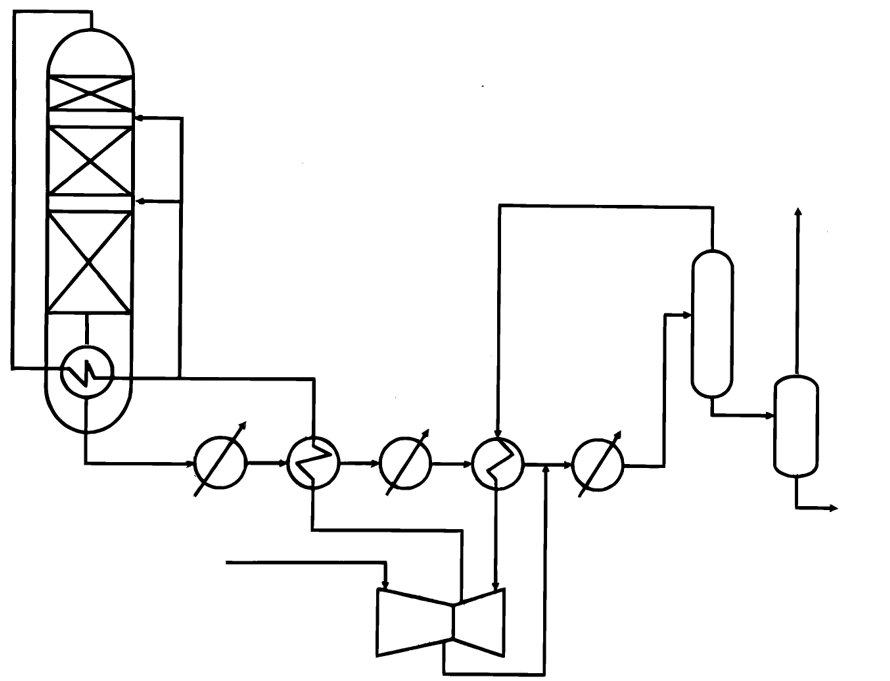
\includegraphics[width=0.7\textwidth]{figures/amoniak.png}};
\node[font=\small,align=right] at (-3.85,-2.52) {amoniak\\syntézní plyn};
\node[font=\small] at (0.3,-4.2) {kompresor/expandér};
\node[font=\small,align=right] at (3.74,-2.46) {tekutý\\amoniak};
\node[font=\small,align=center] at (3.75,2.1) {nezkonvertovaný\\syntézní plyn};
\node[font=\scriptsize] at (-2.5,-0.65) {voda};

\node[font=\scriptsize] at (-2.45,-0.2) {$150 \mathrm{^{\circ}C}$};
\node[font=\scriptsize] at (-4.5,-1.15) {$330 \mathrm{^{\circ}C}$};
\node[font=\tiny] at (-3.9,3.1) {$400 \mathrm{^{\circ}C}$};
\node[font=\tiny] at (-3.96,0.13) {$470\ \mathrm{^{\circ}C}$};
\node[font=\scriptsize] at (0.12,-0.7) {$40 \mathrm{^{\circ}C}$};
\node[font=\scriptsize] at (2.2,0.5) {$-6 \mathrm{^{\circ}C}$};
\end{tikzpicture}
    \caption[Schéma Haber-Boschova procesu syntézy amoniaku]{Schéma Haber-Boschova procesu syntézy amoniaku \cite{Seddon2022}.} \label{fig:amoniak}
\end{figure} 

\subsection{Výroba metanolu}
Metanol (\ce{CH3OH}) je nejjednodušší sloučeninou ze skupiny alkoholů, která se v chemickém průmyslu využívá na výrobu formaldehydu a kyseliny octové, nebo jako aditivum do paliv. Obecně tedy metanol slouží jako surovina, nebo rozpouštědlo pro další chemické procesy. \cite{Seddon2022,Basile2017}

Výroba metanolu se realizuje za využití následující exotermní reakce \cite{Seddon2022}
\reaction{CO + 2H2 -> CH3OH}
Syntézní plyn je před průchodem konvertorem stlačen na $\approx10\ \mathrm{MPa}$ a ohřán na $\approx250\ \mathrm{^{\circ}C}$ a za působení katalyzátorů je syntézní plyn konvertován na metanol. \cite{Seddon2022}

Obdobně jako amoniaku, metanol lze využít jako potenciální \enquote{nosič} čistého vodíku pro palivové články a paliva obecně. Jeho separování probíhá parním reformingem metanolu (s příměsí vody), pří kterém vzniká vodík a oxid uhličitý. \cite{Seddon2022} Při diskuzi o vodíkovém hospodářství, probíraném dále v práci, je fakt využití alternativních nosičů vodíku důležitý pro rozvoj vodíkové infrastruktury.

\section{Využití v metalurgickém průmyslu}
Kvůli dobré reaktivitě vodíku jej lze využívat i v metalurgickém průmyslu, přesněji jako reaktantu při žíhání. Ohřívaný vodík společně s kyslíkem (\ce{O2}) vyvolají chemickou reakci, jejíž produktem je voda. Oxidačně redukční potenciál vody je pak oproti samotnému kyslíku výrazně menší a tedy pro tepelně zpracovávanou součást méně škodlivější. \cite{Ramachandran1998}

Větší uplatnění pak vodík našel v dekarbonizaci výroby ocelí přímou redukcí železné rudy zeleným vodíkem (\acs{DRI}). Tím se rozumí přeměna železné rudy (nejčastěji ve formě hematitu \ce{Fe2O3}) na čisté železo (\ce{Fe}) bez přeměny na kapalnou fázi. Odstraněním kyslíku z železné rudy lze docílit za použití reakčních činidel, kterými mohou být buď oxid uhelnatý (\ce{CO}), nebo právě vodík. Rychlost redukční reakce je pak vyšší při použití čistého vodíku, než oxidu uhelnatého nebo jejich sloučeniny ve formě syntetického plynu. Redukční reakce, uvedené v následujících rovnicích, jsou endotermní a tedy je nutné k jejich průběhu dodat tepelnou energii. V celém procesu se pak teplota pohybuje mezi $700 \div 900^{\circ}\mathrm{C}$. \cite{Bhaskar2020}
\reaction{3 Fe2O3 (s) + H2 (g) -> 2 Fe3O4 (s) + H2O (g)}
\reaction{Fe3O4 (s) + H2 (g) -> 3 FeO (s) + H2O (g)}
\reaction{FeO (s) + H2 (g) ->  Fe (s) + H2O (g)}
Na výrobu železa metodou \acs{DRI} používají šachtové a rotační pece případně rotační ohniště, nebo reaktory s fluidní vrstvou. Šachtové pece pak fungují jako protiproudé reaktory s pohyblivým ložem. Rotační pece se používají v případě, kdy zdroj pro výrobu redukčních plynů je uhlí. \cite{Bhaskar2020}

K přímé redukci železné rudy se využívá až 10$\%$ veškerého vyrobeného vodíku ve formě sloučenin, což odpovídá přibližně $4\ \mathrm{Mt_{H_2}}$ za rok, viz. graf na Obr. \ref{fig:pouziti_vodiku_proc}. \cite{IEAfuture} Využití zeleného vodíku dává metalurgickému průmyslu, který se podílí ze $7\%$ na celosvětové produkci emisí oxidu uhličitého, potenciál snížit emise až o $2,3\ \mathrm{Gt_{CO_2}}$ za rok. Překážkou rozvoje této technologie je však aktuální vysoká cena zeleného vodíku, která má za důsledek vyšší finanční náročnost celého procesu oproti konvenčnějším výrobám železa, popř. oceli. \cite{Bhaskar2020}

\section{Využití v dopravním sektoru}
Paliva na bázi vodíku, nebo vodík samotný, lze dále použít jako potencionální palivo do nákladních lodí, letadel, nebo automobilů. Obměna současných technologií pohánění dopravních prostředků pomocí vodíkových technologií je z důvodu nedostatečné připravenosti infrastruktury dlouhodobou vizí dekarbonizace tohoto odvětví.

Až $90\%$ přepravy veškerých komodit, z čehož třetinu tvoří ropné produkty a paliva, je realizováno námořní dopravou. Emise skleníkových plynů tohoto sektoru tvoří až $3\%$ podíl z veškerých světových emisí ($\approx0,9\ \mathrm{Gt_{CO_2}}$ za rok). Nahrazení fosilních paliv v námořní dopravě palivy na bázi vodíku je zatím omezeno na experimentální zkoumání s předpokládaným částečným nahrazením v horizontu $10$ let. \cite{Griffiths2021,Bouman2017}

V osobních a nákladních automobilech lze využít vodík pro jejich pohon ve dvou variantách. V první variantě dochází ke spalování v komoře, obdobně jako v tradičních spalovacích motorech. Druhá konstrukční varianta spočívá v transformaci energie v tzv. palivových článcích (\acs{FC}), kde přiváděný vodík reaguje s kyslíkem a elektrochemickou reakcí vzniká voda a energie ve formě elektřiny a tepla. \cite{Hytep,Mekhilef2012,Turon2020}
\reaction{2H2 (g) + O2 (g) -> 2H2O + energie}
Ve své podstatě se jedná o reverzní elektrolýzu, kdy na anodě vodík oxiduje na
na protony a elektrony, zatímco na katodě kyslík redukuje na oxidy a za přítomnosti protonů vodíku z katody vzniká voda. Elektrická energie vyráběna v palivových článcích se následně ukládá do systému baterií uložených pod podvozkem automobilu. Elektrické motory pak přímo odebírají elektrický proud z bateriových systémů a tím pohání vozidlo. Takto fungující vozidlo je pak označováno jako elektromobil s palivovými články (\acs{FCEV}), které je znázorněno na Obr. \ref{fig:fcev}. \cite{Mekhilef2012}
\begin{figure}[h]
    \centering
    \begin{tikzpicture}
\node[inner sep=0pt] (obrazek) at (0,0)
    {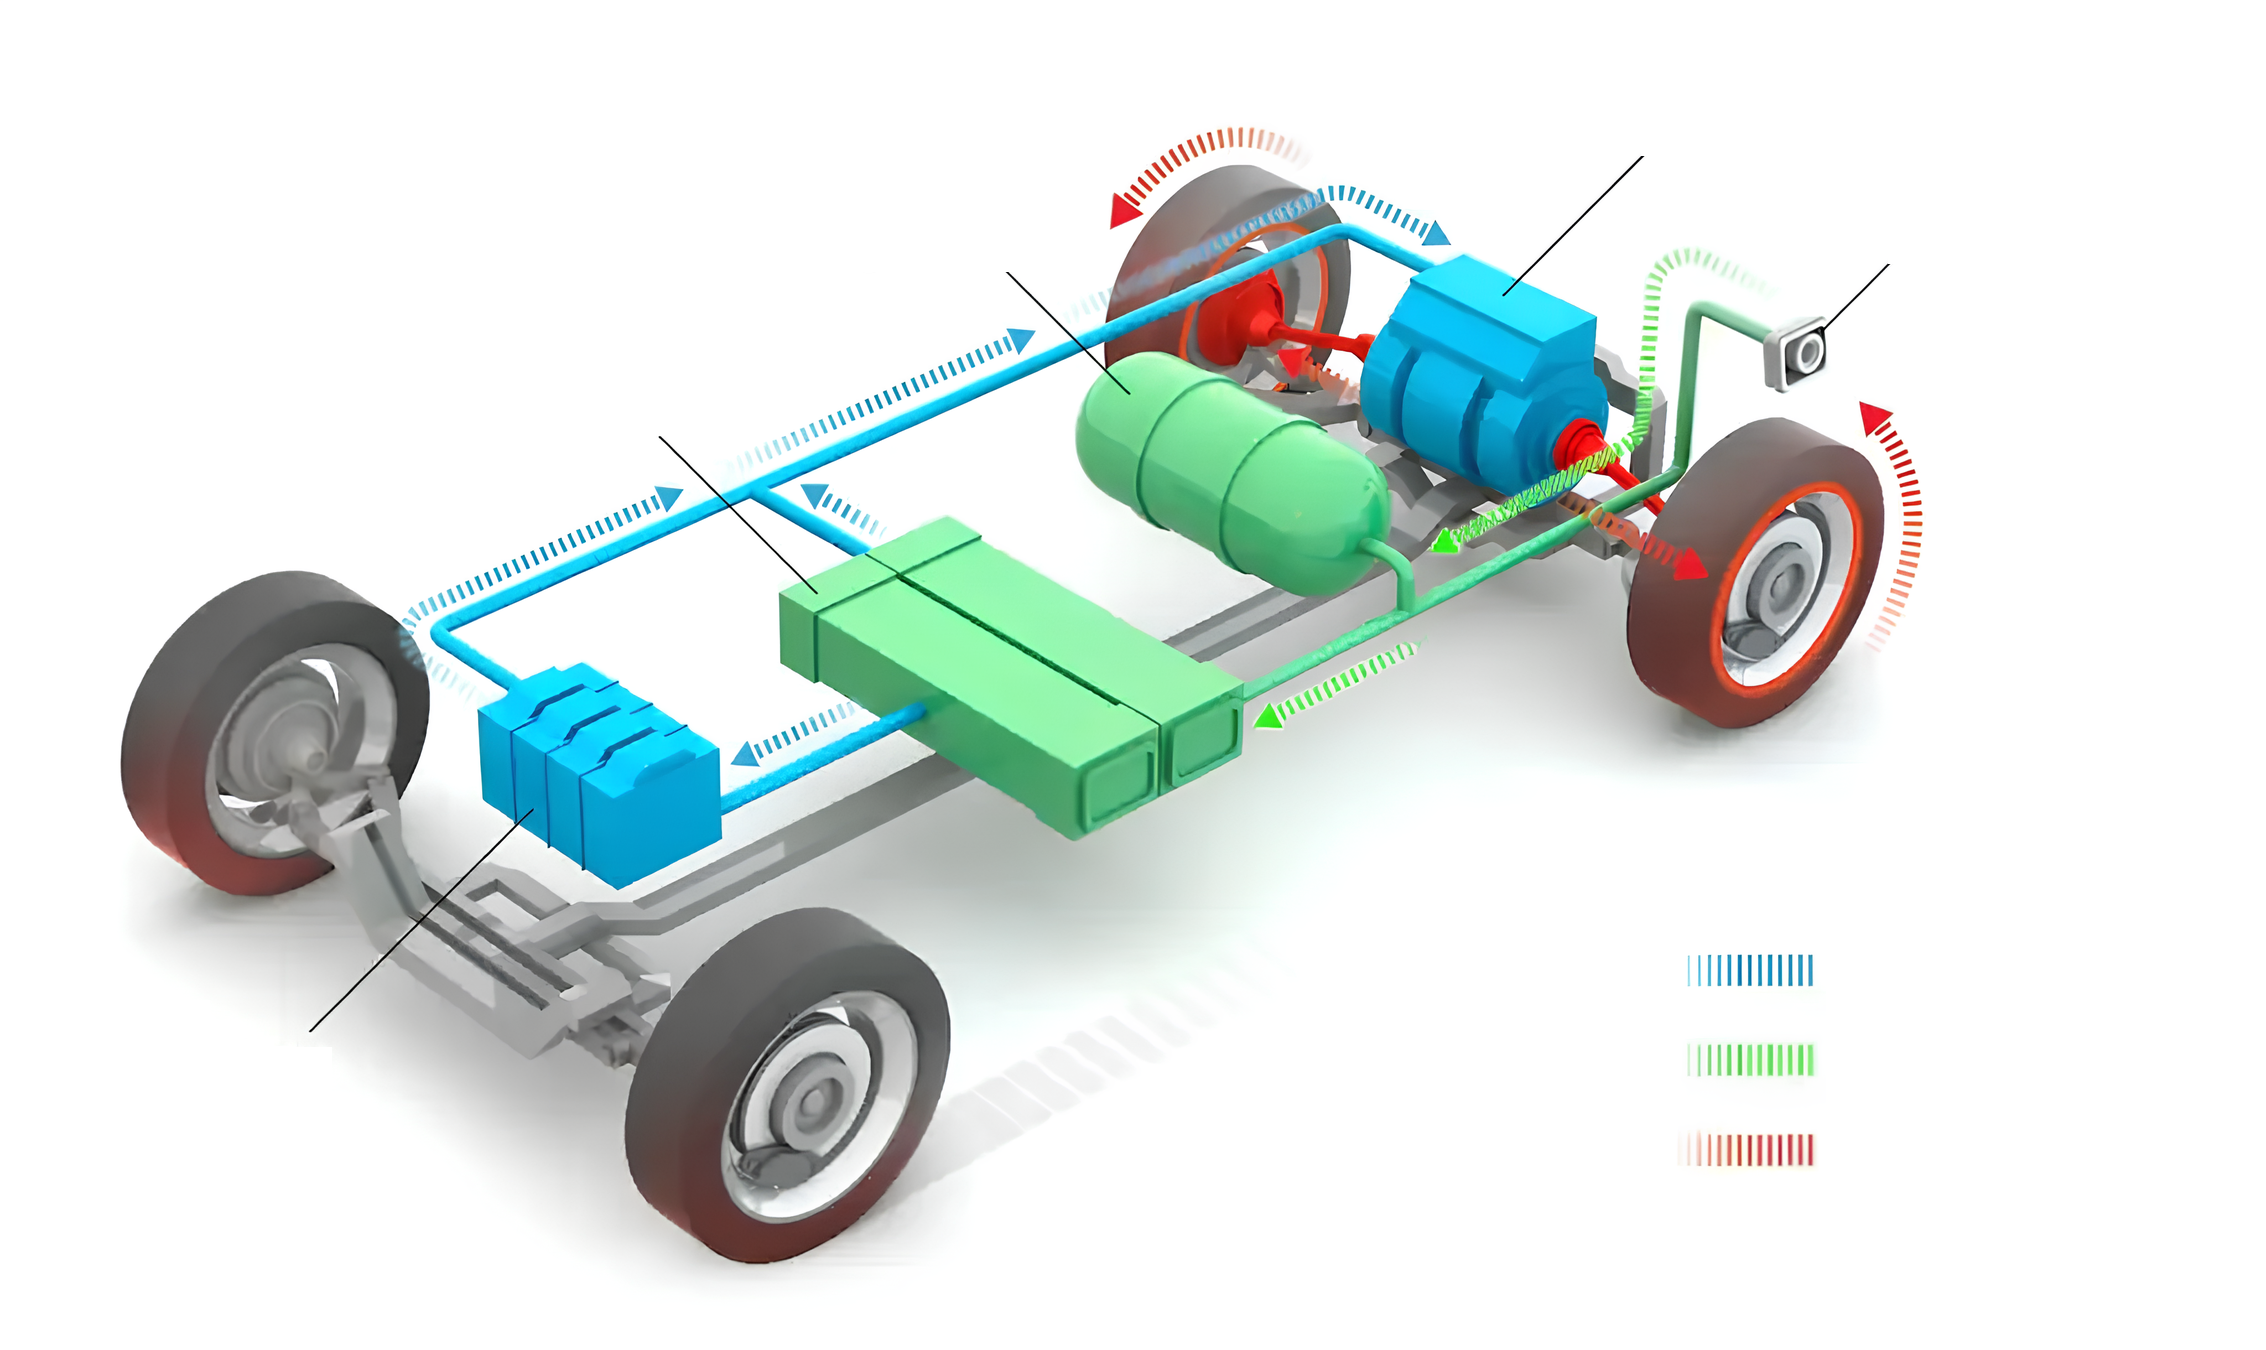
\includegraphics[width=0.8\textwidth]{figures/fcev.png}};
\node[font=\footnotesize] at (4.8,-1.52) {Elektrická energie};
\node[font=\footnotesize] at (3.95,-1.92) {Vodík};
\node[font=\footnotesize] at (4,-2.35) {Pohon};
\node[font=\small] at (5.55,2.1) {Hrdlo palivové nádrže};
\node[font=\small] at (3.95,2.65) {Elektrický motor};
\node[font=\small] at (-1.9,2.2) {Nádrž na vodík};
\node[font=\small] at (-3.2,1.4) {Palivový článek};
\node[font=\small] at (-4.4,-2) {Baterie};
\end{tikzpicture}
    \caption[Schéma elektromobilu s palivovým článkem]{Schéma elektromobilu s palivovým článkem, převzato z \cite{Arif2023}.} \label{fig:fcev}
\end{figure}

Účinnost celého systému se pohybuje mezi $40\div50\%$, což je sice méně než u běžných bateriových elektromobilů (BEV), ale i přesto dokáže konkurovat vozidlům poháněným běžnými spalovacími motory (ICE), kde se účinnost pohybuje mezi $25\div40\%$. \cite{Hytep,Mekhilef2012,Turon2020} Mezi hlavní výhody používání FCEV se řadí nevypouštění znečišťujících látek do životního prostředí a vysoký dojezd konkurující vozidlům vybaveným běžným spalovacím motorem ($\approx 600\ \mathrm{km}$). Nevýhodami pak jsou vysoká pořizovací cena automobilu (až o $50\%$ vyšší než vozidla se spalovacími motory) a nedostatečná infrastruktura plnících stanic pro tankování. \cite{Hytep,Turon2020}

\section{Využití v rafinérském průmyslu}
\label{sec:vyuziti_raf}

Vodík je nedílnou součástí široké škály procesů i v rafinérském odvětví, kde se jeho využití rozšiřuje do mnoha procesů, od úpravy paliv po jejich výrobu. Necelých $38\ \mathrm{Mt_{H_2}}$ za rok, tj. $33\%$ celkové celosvětové poptávky po vodíku (v čisté formě i sloučeninách), spotřebují rafinerie buď jako surovinu, reaktant, nebo nosič energie, viz. Obr. \ref{fig:pouziti_vodiku_proc}. \cite{IEAfuture}. Při pohledu na současný stav a budoucí trendy je zřejmé, že vodík hraje klíčovou roli při transformaci rafinérského průmyslu směrem k udržitelnějšímu a energeticky efektivnějšímu. Poptávka rafinerií po vodíku se tak bude i nadále zvyšovat a se zpřísňováním předpisů týkajících se obsahu síry v ropných produktech bude kladen důraz na jeho využívání. \cite{Blazek2006} 

Vodík je v rafineriích po celém světě nejvíce využíván jako reaktant v hydroprocesech, což je souhrnný název pro technologie krakování, hydrogenace apod. \cite{Speight2020} Kvůli dobré reaktivitě vodíku je vhodné jej využít i na odstranění nečistot konečných produktů. Tyto procesy mohou být například hydrodesulfurace, nebo hydrodenitrogenace, obecně tedy hydrogenační rafinace. Tyto i další aplikace jsou popsány v následujících podkapitolách.

\subsection{Přeměny těžkých ropných frakcí}
\label{subsec:premenytrp}

Pro úplné pochopení probírané tématiky a rozeznání rozdílů je nutné zadefinovat základní používané názvy:
\begin{description}[style=unboxed,leftmargin=0cm]
\item[Těžké ropné frakce] jsou produktem frakční destilace ropy za vyšších teplot. Jsou charakteristické jejich malým poměrem \ce{H/C}\footnote{Poměr vodíku ku uhlíku v uhlovodících, tedy organických sloučeninách pouze atomů vodíku a uhlíku, získávaných rafinací ropy.} a velkým obsahem uhlíku. Mezi těžké ropné frakce patří např. topné oleje, mazací oleje, asfalt apod. \cite{Blazek2006}
\item[Lehké ropné frakce] jsou obdobně jako těžké ropné frakce získávány pomocí destilace ropy (atmosferické i vakuové), avšak destilační rozmezí teplot jejich produkce je menší. Mají větší poměr \ce{H/C} a zároveň výrazně méně atomů uhlíku (v řádu jednotek). Za lehké frakce bývají označovány rafinérské plyny a automobilové benziny, ale také motorová nafta, či letecký petrolej. \cite{Blazek2006}
\item[Katalyzátor] je látka zvyšující rychlost a pravděpodobnost vzniku reakce, ale z které sama vychází nezměněná, nespotřebovaná. Katalyzátory zároveň neovlivňují termodynamickou rovnováhu reakce a dosahují požadovaných přeměn s nižší energetickou náročností prostřednictvím alternativního mechanismu. \cite{Bartovska2016}
\end{description}
Pro naplnění stále zvyšující se poptávky po pohonných hmotách je v rafinériích nutné zpracovávat ropu ve velkém objemu. Vzhledem k složení ropy dochází k nedostatku vyrobených lehkých frakcí, které se používají jako paliva a zároveň nadbytku těžkých frakcí, kterých se celosvětově spotřebuje až o polovinu méně. \cite{Blazek2006} Pro získání většího množství lehkých frakcí lze těžké ropné frakce dále štěpit a zpracovávat.

\subsubsection{Katalytické hydrokrakování}

Krakovacími procesy obecně rozumíme štěpení těžkých frakcí na lehké frakce. Toho dosáhneme buď termickým, katalytickým, nebo \textbf{katalytickým hydrogenačním krakováním}, zkráceně nazývaného \textbf{hydrokrakování}. Princip termického krakování (koksování, visbreaking) spočívá v štěpení molekul uhlovodíku pouze teplem, kdežto u katalytického krakování vedle tepla působí i katalyzátory. Základ katalyzátorů v procesech fluidního i termoforového katalytického krakování tvoří aluminosilikáty (hlinitokřemičitany), které mají vysokou tepelnou odolnost, až $400\ \mathrm{^{\circ}C}$. \cite{Blazek2006} Využívané katalyzátory tvoří iontové reakce, za kterých jsou z uhlovodíků vytvářeny karboniové ionty, podléhající sekundární reakci štěpení uhlíkových vazeb. \cite{Bartovska2016}

\paragraph{Historie, vývoj a aplikace}
V první polovině minulého století se s rozvojem automobilového průmyslu začaly více zvyšovat požadavky na kvalitu motorových paliv. Paliva získaná katalytickým krakováním však těmto požadavkům přestávaly vyhovovat a s tím se podnítil rozvoj obecně účinnější  technologie hydrokrakování, kdy byl do reakce přiváděn vodík. Jedním z prvních rafinérských závodů, kde se hydrokrakování uplatnilo byl uveden do provozu v roce 1927 ve východoněmeckém městě Leuna. \cite{Speight2020} Hydrogenace hnědého uhlí a hnědouhelného dehtu byla prováděna především pro komerční účely a kapacita výroby konečných produktů činila ve válečných letech až $600\ 000$ tun ročně. Z konečných produktů bylo $60\%$ leteckého a automobilového benzinu a $40\%$ motorové nafty. \cite{Holroyd1945} Jako katalyzátor byl v jednostupňové jednotce použit sulfid wolframu (\ce{WS2}). Za vysokých reakčních tlaků ($\approx 20 \div 30\ \mathrm{MPa}$) katalyzátor vykazoval velmi vysokou účinnost, kdy uhlí, dusík a kyslík a ostatní vstupní suroviny byly prakticky zcela převedeny na lehké frakce. V druhé polovině 20. století se procesy hydrokrakování staly ekonomicky výhodnějšími kvůli změně a zdokonalení používaných katalyzátorů. To umožnilo zařízením pracovat při podstatně nižších tlacích, v rozmezí přibližně $7 \div 15\ \mathrm{MPa}$. \cite{Speight2020}

Hydrokrakování lze kromě zpracování těžkých frakcí na motorový benzin, naftu, petrolej a topné oleje využít také na výrobu hydrogenovaného vakuového destilátu\footnote{Tento proces je také často nazýván \enquote{mírné hydrokrakování}.}, který slouží jako vstupní surovina pro výrobu mazacích olejů. Průběh těchto dvou procesů se liší ve výstupu z frakční kolony. U mírného hydrokrakování je produktem olejový hydrokrakát, který dále putuje do jednotky vakuové destilace, v které jsou formovány mazací oleje. \cite{Blazek2006}

\paragraph{Chemické reakce a jejich podmínky}
Při hydrokrakování jsou stejně jako při katalytickém krakování meziproduktem iontové reakce karboniové ionty, které jsou hydrogenovány za vysokých parciálních tlaků vodíku a následnými sekundárními reakcemi štěpeny za vzniku nízkomolekulárních produktů. Celý proces je pak nerozvětvenou řetězovou reakcí, která je velmi rozsáhlá. \cite{Speight2020} V této práci bude upřednostněn popis samotného procesu fungování hydrokrakovacího zařízení, které může být buď jedno, nebo dvou stupňové.

Hlavní parametry probíhajících reakcí, jež mají vliv na konverzi\footnote{Konverze suroviny $[\mathrm{hm.}\%]$ je v krakovacích procesech vyjádřena jako výtěžek produktů, které mají bod varu nižší než bod varu nejtěžší složky, která je získávána ve frakční koloně. \cite{Blazek2006}} vstupní suroviny jsou reakční teplota, tlak, poměr vodíku a suroviny a objemová rychlost. Data jsou převzata z publikace \cite{Blazek2006} a uvedeny v Tab. \ref{tab:rp_hydrokrakovani}.
\begin{table}[h]
    \centering
    \begin{tabular}{|c|c|}
        \hline
        \textbf{Parametr reakce} & \textbf{Hodnoty a jednotky} \\ \hline\hline
        Teplota & $350\div450\ \mathrm{^{\circ}C}$ \\ \hline
        Tlak & $5 \div 20\ \mathrm{MPa}$ \\ \hline
        Poměr vodíku a suroviny & $500 \div 1500\ \mathrm{m^3_{suroviny}/m^3_{\ce{H2}}}$ \\ \hline
        Objemová rychlost & $0,5 \div 2\ \mathrm{m^3_{suroviny}/h}$ na $1\ \mathrm{m^3_{\text{katalyzátoru}}}$ \\ \hline
    \end{tabular}
    \caption[Reakční podmínky hydrokrakování]{Reakční podmínky hydrokrakování \cite{Blazek2006}.}
    \label{tab:rp_hydrokrakovani}
\end{table}

\noindent
Hydrokrakování probíhá v relativně intervalu nízkých \textit{teplot}, kvůli využívání katalyzátorů. Ty jsou obdobně jako u katalytického krakování silně kyselé aluminosilikáty, které plní v procesu krakovací, neboli štěpící funkci. Vysoce kyselé katalyzátory jsou však citlivé na dusíkaté sloučeniny v surovině, které za reakčních podmínek rozkládají na amoniak a neutralizují kyselá místa. Hydrogenační reakce v procesu hydrokrakování pak zajišťují sulfidy wolframu, molybdenu, kobaltu, nebo niklu. Tyto aktivní složky pak chrání katalyzátory před kondenzačními reakcemi, které vedou k tvorbě koksu a následnému zpomalování reakce. Tvorba a usazování koksu na katalyzátorech je také omezena velkým \textit{tlakem} při hydrogenačních reakcích, který zároveň zvyšuje konverzi vstupních surovin na lehčí ropné frakce. \cite{Blazek2006,Speight2020}

\subsubsection{Hydrokrakování vakuových destilátů}
\label{subsubsec:hkvd}

Hydrokrakování vakuových destilátů se provádí ve dvou základních konfigurací, z čehož jednostupňová konfigurace hydrokrakovacího zařízení je nejjednodušší z hlediska uspořádání reaktorové části. Hlavním rozdílem mezi jednostupňovým a dvoustupňovým hydrokrakováním je opětovné využití destilačního zbytku vystupujícího z frakční kolony (\textbf{6}) po prvním hydrokrakování. Dvoustupňový proces hydrokrakování se pak využívá převážně za účelem výroby lehkých a těžkých benzinů. \cite{Blazek2006} Celé schéma níže popsaných procesů je graficky znázorněno na Obr. \ref{fig:hydrokrak_2schema} i s oddělením procesů.
\begin{figure}[h]
    \centering
    \begin{tikzpicture}
\node[inner sep=0pt] (obrazek) at (0,0)
    {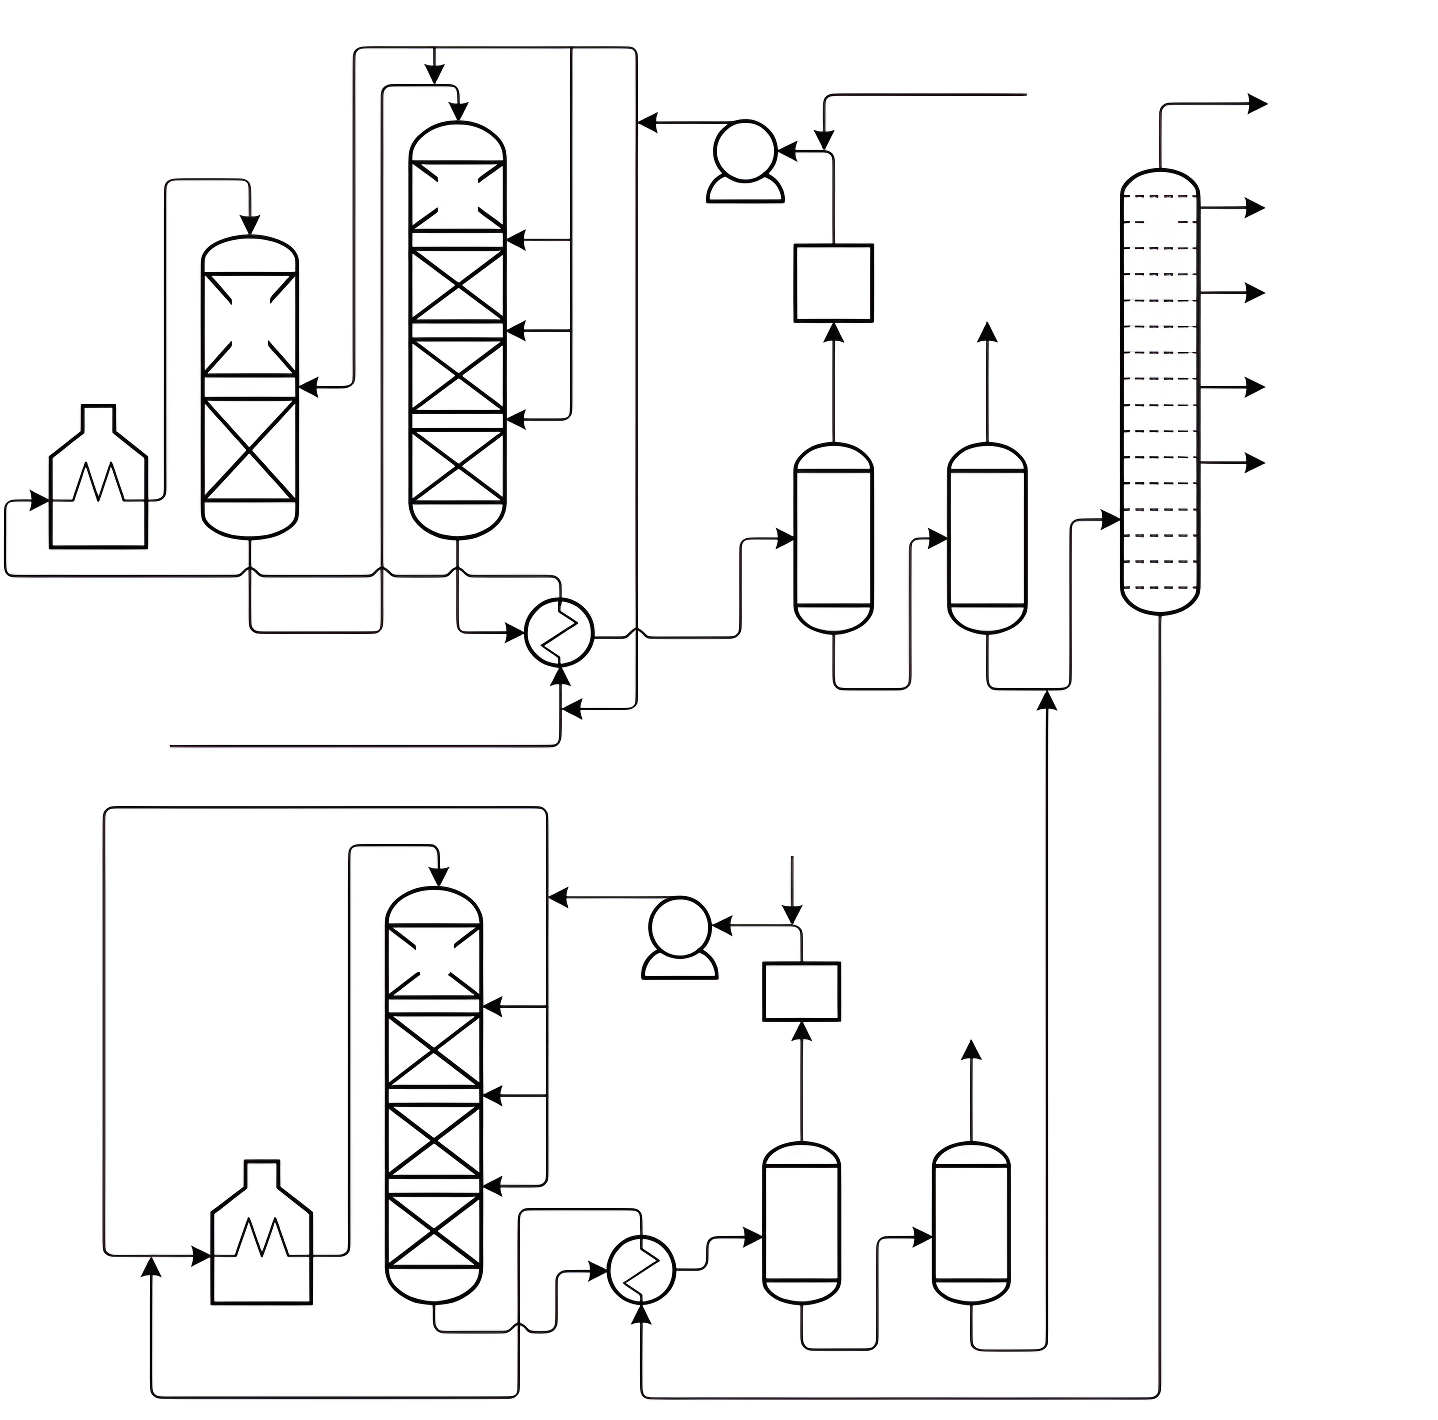
\includegraphics[width=0.77\textwidth]{figures/hydrokrak_2schema.png}};
\node[font=\small\bfseries] at (-4.65,1.4) {1};
\node[font=\small\bfseries] at (-3.52,2.92) {2};
\node[font=\small\bfseries] at (-1.97,3.85) {3};
\node[font=\small\bfseries] at (0.85,1.55) {4};
\node[font=\small\bfseries] at (2,1.55) {5};
\node[font=\small\bfseries] at (3.31,3.65) {6};
\node[font=\small\bfseries] at (0.85,3.2) {7};
\node[font=\small\bfseries] at (0.195,4.2) {8};

\node[font=\scriptsize] at (-2.95,2.7) {\ce{H2}}; % u 2
\node[font=\scriptsize] at (-1.75,4.8) {\ce{H2}}; % nad 3
\node[font=\scriptsize] at (-0.85,0.2) {\ce{H2}}; % nalevo od 4
\node[font=\scriptsize] at (-4.3,-2.5) {\ce{H2}}; % nad 1 v druhém stupni
\node[font=\scriptsize,align=left] at (2.4,2.4) {\ce{H2S\\NH3}};

\node[font=\small] at (-4.9,-0.25) {surovina};
\node[font=\small,align=center] at (0.2,2.35) {recykl\\\ce{H2}};
\node[font=\small] at (1.94,3.15) {plyny};
\node[font=\small] at (1.55,4.84) {čerstvý \ce{H2}};
\node[font=\scriptsize] at (0.61,-0.23) {recykl vakuového destilátu};

\node[font=\small] at (4.7,4.6) {plyny};
\node[font=\small,align=left] at (4.785,3.9) {lehký\\benzin};
\node[font=\small,align=left] at (4.785,3.1) {těžký\\benzin};
\node[font=\small] at (4.865,2.45) {petrolej};
\node[font=\small,align=left] at (4.88,1.8) {plynový\\olej};
\node[font=\small,align=left] at (4.88,0.5) {vakuový\\destilát};

\draw[dashed] (3.4,0.7) -- (3.4,-0.4);
\draw[dashed] (3.4,-0.4) -- (-3,-0.4);
\draw[->,dashed] (-3,-0.4) -- (-3,0.57);
\draw[->,dashed] (3.4,0.5) -- (4.121,0.5);

\node[font=\small,align=left] at (4.2,-2) {destilační\\zbytek};
\node[font=\footnotesize] at (-2.9,-4.95) {destilační zbytek};
\node[font=\small] at (1.94,-2.22) {plyny};
\node[font=\small] at (0.61,-0.9) {čerstvý \ce{H2}};
\node[font=\small,align=center] at (0,-2.85) {recykl\\\ce{H2}};

\node[font=\small\bfseries] at (-3.45,-4.25) {1};
\node[font=\small\bfseries] at (-2.125,-1.85) {3};
\node[font=\small\bfseries] at (0.6,-3.65) {4};
\node[font=\small\bfseries] at (1.89,-3.65) {5};
\node[font=\small\bfseries] at (0.6,-2.1) {7};
\node[font=\small\bfseries] at (-0.3,-1.62) {8};

\draw[decoration={calligraphic brace,amplitude=5pt}, decorate, line width=1.25pt] (-5.8,-0.5) -- (-5.8,5);
\draw[decoration={calligraphic brace,amplitude=5pt}, decorate, line width=1.25pt] (-5.8,-5.2) -- (-5.8,-0.7);
\node[font=\small\bfseries,rotate=90] at (-6.3,2.35) {První stupeň};
\node[font=\small\bfseries,rotate=90] at (-6.3,-2.9) {Druhý stupeň};
\end{tikzpicture}
    \caption[Schéma jednostupňového a dvoustupňového hydrokrakování]{Schéma jednostupňového a dvoustupňového hydrokrakování \cite{Blazek2006}.\\(1 - pec, 2 - hydrogenační reaktor, 3 - hydrokrakovací reaktor, 4 - vysokotlaký separátor, 5 - nízkotlaký separátor, 6 - frakční kolona, 7 - vypírka kyselých plynů, 8 - vodíkový kompresor)} \label{fig:hydrokrak_2schema}
\end{figure}

V první fázi procesu se surovina v podobě vakuových destilátů smísí s recyklovaným přebytkem vodíku a po předehřátí (\textbf{1}) na požadovanou teplotu vstupuje do hydrogenačního reaktoru prvního stupně (\textbf{2}). V reaktoru dochází za působení katalyzátorů k desulfuračním a denitrogenačním exotermním reakcím. Po výstupu uhlovodíků z hydrogenačního reaktoru, je před dalším procesem nutné chlazení, které se provádí vháněním chladicích plynů mezi lože katalyzátoru. Poté již následuje nástřik do hydrokrakovacího reaktoru (\textbf{3}), kde probíhají výše zmíněné chemické reakce hydrokrakování. Vystupující zkapalněné uhlovodíky dále vstupují do dvojice vysokotlakého (\textbf{4}) a nízkotlakého separátoru (\textbf{5}). Ve vysokotlakém separátoru dochází k uvolňování přebytku vodíku a jeho recyklaci zpět do oběhu na začátek procesu. V nízkotlakém separátoru dochází k odstranění nežádoucích plynů z produktu, jako je sirovodík a amoniak. Poté již následuje průchod produktu přes frakční kolonu (\textbf{6}), kde se dělí na plyny, lehké a těžké benziny, petrolej, plynový olej a lehký vakuový destilát, který se obdobně jako přebytečný vodík vhání zpět do reaktoru. \cite{Blazek2006,Speight2020} 

V druhém stupni hydrokrakovací jednotky pak není obsažen hydrogenační reaktor kvůli nízkému obsahu již vyseparovaných sirných a dusíkatých složek. Separace výstupních uhlovodíků pak probíhá společně ve frakční koloně (\textbf{6}) s produkty z prvního hydrokrakovacího reaktoru. \cite{Blazek2006}

Tyto konfigurace našly uplatnění v případech, kdy je požadována konverze suroviny na jeden průchod v intervalu $40\div70\ \mathrm{hm.}\%$ a kde je požadavek na zpracovávaní vakuového destilátu na paliva a na hydrogenovaný vakuový zbytek, který se dále používá v procesech fluidního katalytického krakování. \cite{Blazek2006}
\begin{figure}[h]
    \centering
    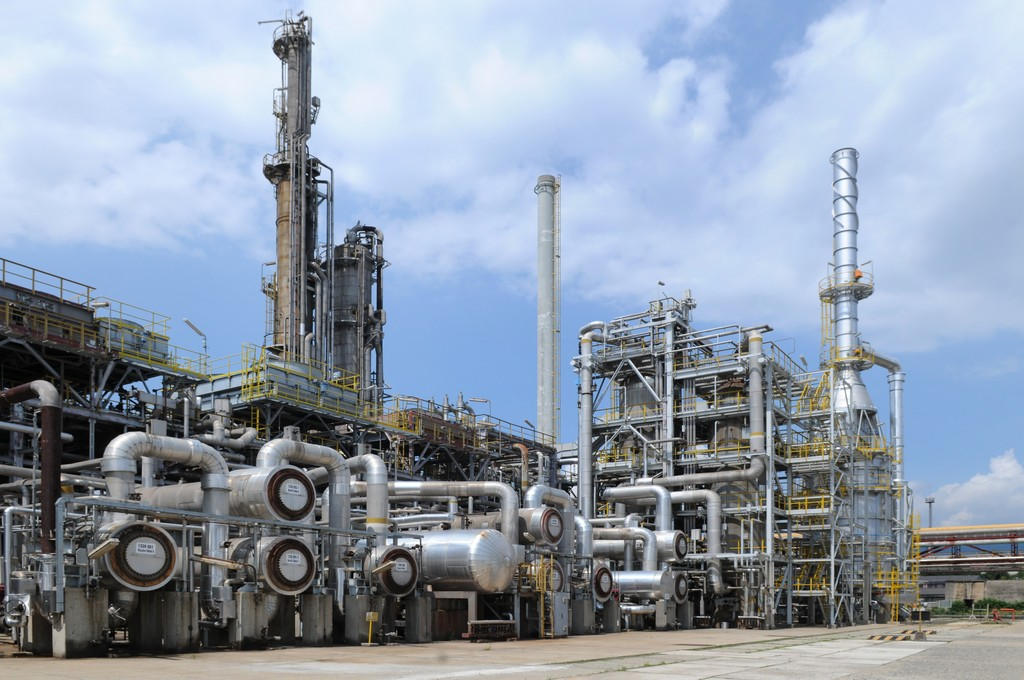
\includegraphics[width=.6\textwidth]{figures/hydrokrak_litvinov.jpg}
    \caption[Hydrokrakovací jednotka v Litvínově - Záluží]{Hydrokrakovací jednotka v Litvínově - Záluží \cite{hydrokrak_litvinov}.} \label{fig:hydrokrak_litvinov}
\end{figure}

Hydrokrakovací jednotku provozuje v České republice firma \textit{Orlen Unipetrol RPA s.r.o.} (dříve \textit{Česká rafinérská a.s.}) v Litvínově - Záluží. Jednotka na Obr. \ref{fig:hydrokrak_litvinov}, je dimenzovaná na výkon až $160\ \mathrm{t_{\text{produktů}}/}$hodinu a konečnou konverzí pohybující se v rozsahu $41 \div 74\ \mathrm{hm.}\%$. \cite{HKlitvinov}

\subsubsection{Hydrokrakování vakuových zbytků}

Rozdíl mezi procesy hydrokrakování vakuových destilátů a vakuových zbytků spočívá především ve volbě vstupní suroviny a konstrukci reaktorů. Suroviny - vakuové zbytky jsou velmi těžké ropné frakce (např. mazut) vystupující z vakuové destilace ropy, které obsahují zbytky kovů (nejčastěji vanad, nikl a železo) a atomy síry, dusíku a kyslíku. Tyto prvky by v reaktorech, zmiňovaných v přecházející kapitole, způsobovaly tzv. deaktivování katalyzátorů\footnote{Deaktivací katalyzátoru rozumíme usazování nečistot v podobně kovů a uvolňovaných uhlíkatých částí na povrchu katalyzátorových loží (koksování). \cite{Blazek2006}}, kvůli kterému by bylo nutné často provádět odstávky jednotek za účelem regenerace, nebo výměny katalyzátorů. \cite{Blazek2006,Prajapati2021}

Konstrukce hydrokrakovacích reaktorů se nejčastěji provádí ve konfiguraci s pevným ložem katalyzátoru a s ložem fluidním. U první varianty jsou před hlavní hydrokrakovací reaktory umístěny tzv. ochranné reaktory, které slouží k částečnému odbourávání katalyzátorům škodících látek. Ochranné reaktory se pak umisťují zpravidla ve dvojici, kdy jeden plní funkci produkční a druhý je záložní. K přepnutí nástřiku suroviny do záložního reaktoru dojde tehdy, kdy je plně deaktivován katalyzátor produkčního (primárního) reaktoru. V mezičase se katalyzátor produkčního reaktoru vymění, nebo regeneruje. Po výstupu z ochranných reaktorů se již jedná o stejný proces jako hydrokrakování vakuových destilátů s výjimkou toho, že ropná frakce prochází dvojicí hydrokrakovacích reaktorů, pro splnění požadované konverze. \cite{Blazek2006}
\begin{figure}[h]
    \centering
    \begin{tikzpicture}
\node[inner sep=0pt] (obrazek) at (0,0)
    {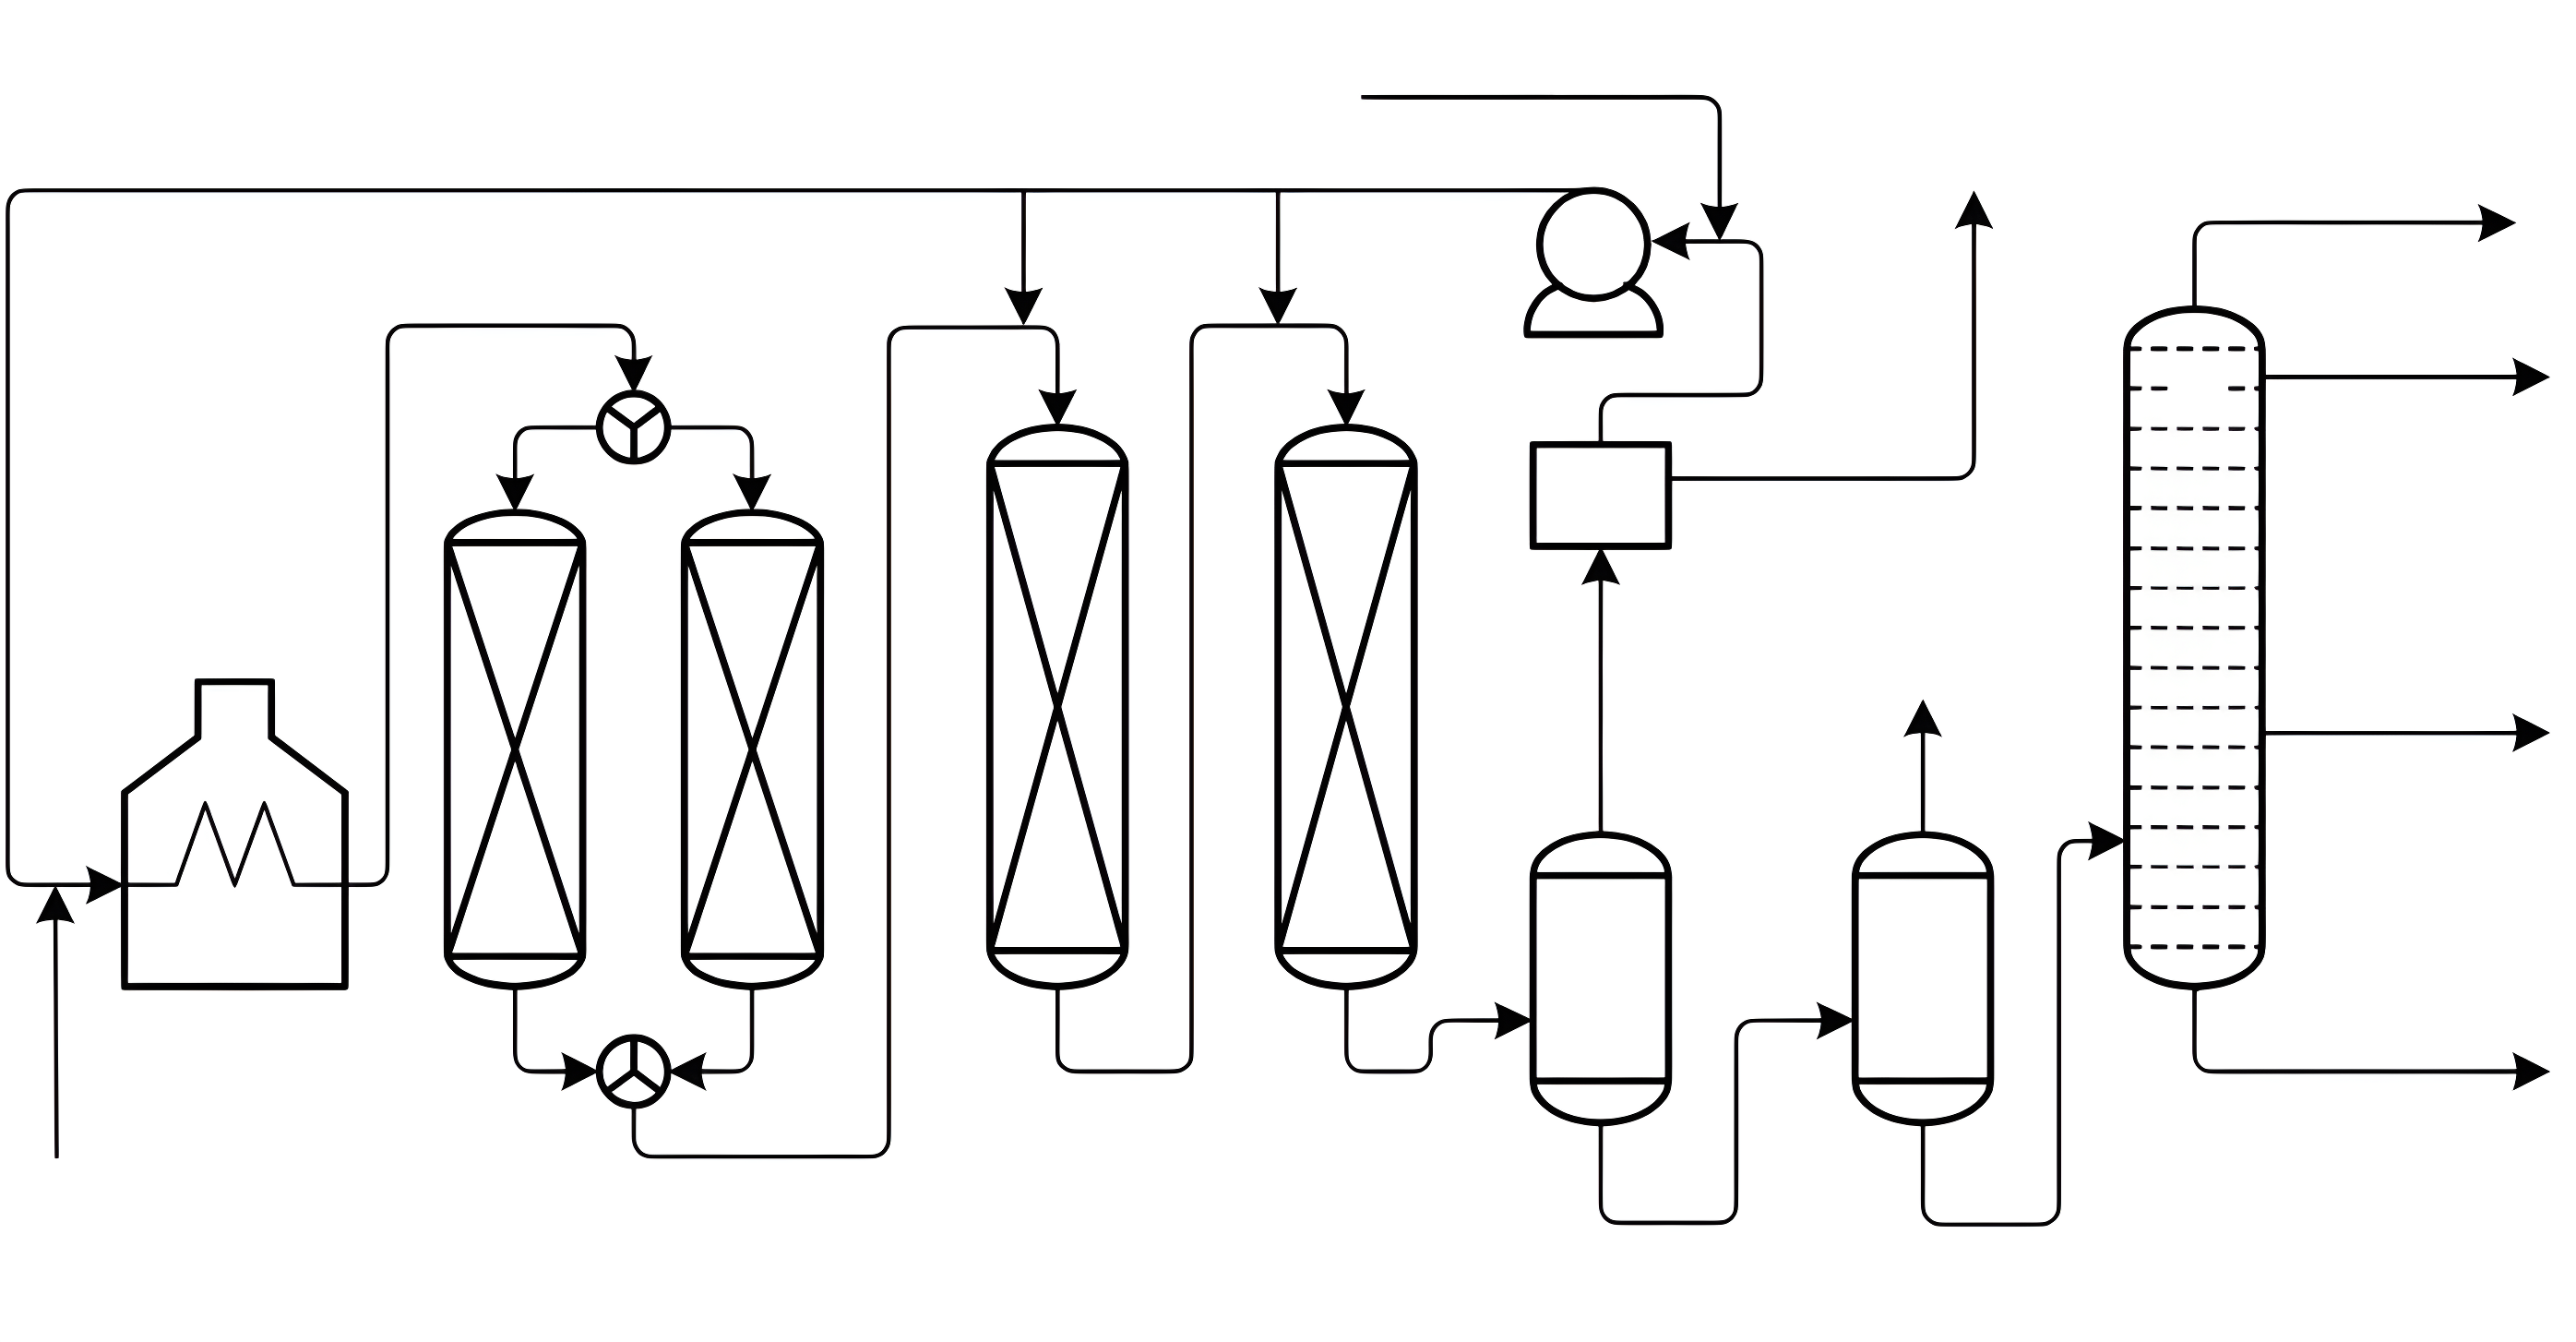
\includegraphics[width=0.8\textwidth]{figures/hydrokrak_Pschema.png}};
\node[font=\small\bfseries] at (-4.57,-1.15) {1};
\node[font=\small\bfseries] at (-3.37,0.317) {2};
\node[font=\small\bfseries] at (-2.3,0.32) {2'};
\node[font=\small\bfseries] at (-1,0.646) {3};
\node[font=\small\bfseries] at (0.25,0.65) {3};
\node[font=\small\bfseries] at (1.35,-1.15) {4};
\node[font=\small\bfseries] at (2.765,-1.15) {5};
\node[font=\small\bfseries] at (3.95,1.22) {6};
\node[font=\small\bfseries] at (1.35,0.77) {7};
\node[font=\small\bfseries] at (1.32,1.85) {8};

\node[font=\scriptsize] at (-2.9,2.3) {\ce{H2}}; % mezi 2 a 2'

\node[font=\small] at (-4.55,-1.97) {surovina};
\node[font=\small] at (-0.6,2.5) {čerstvý \ce{H2}};
\node[font=\small,align=center] at (1.9,-0.3) {recykl\\\ce{H2}};
\node[font=\small] at (2.9,0.15) {plyny};
\node[font=\small,align=center] at (2.9,2.5) {kyselé\\plyny};

\node[font=\small] at (4.8,2.2) {plyny};
\node[font=\small] at (4.8,1.55) {benzin};
\node[font=\small,align=left] at (4.95,0.2) {plynový\\olej};
\node[font=\small,align=left] at (4.65,-2.3) {nízkosirný\\těžký olej};

\end{tikzpicture}
    \caption[Schéma hydrokrakování frakcí v reaktorech s pevným ložem]{Schéma hydrokrakování frakcí v reaktorech \textbf{s pevným ložem} \cite{Blazek2006}.\\(1 - pec, 2 - produkční ochranný reaktor, 2' - záložní ochranný reaktor, 3 - hydrokrakovací reaktory, 4 - vysokotlaký separátor, 5 - nízkotlaký separátor, 6 - frakční kolona, 7 - vypírka kyselých plynů, 8 - vodíkový kompresor)} \label{fig:hydrokrak_Pschema}
\end{figure}
\begin{figure}[ht]
    \centering
    \begin{tikzpicture}
\node[inner sep=0pt] (obrazek) at (0,0)
    {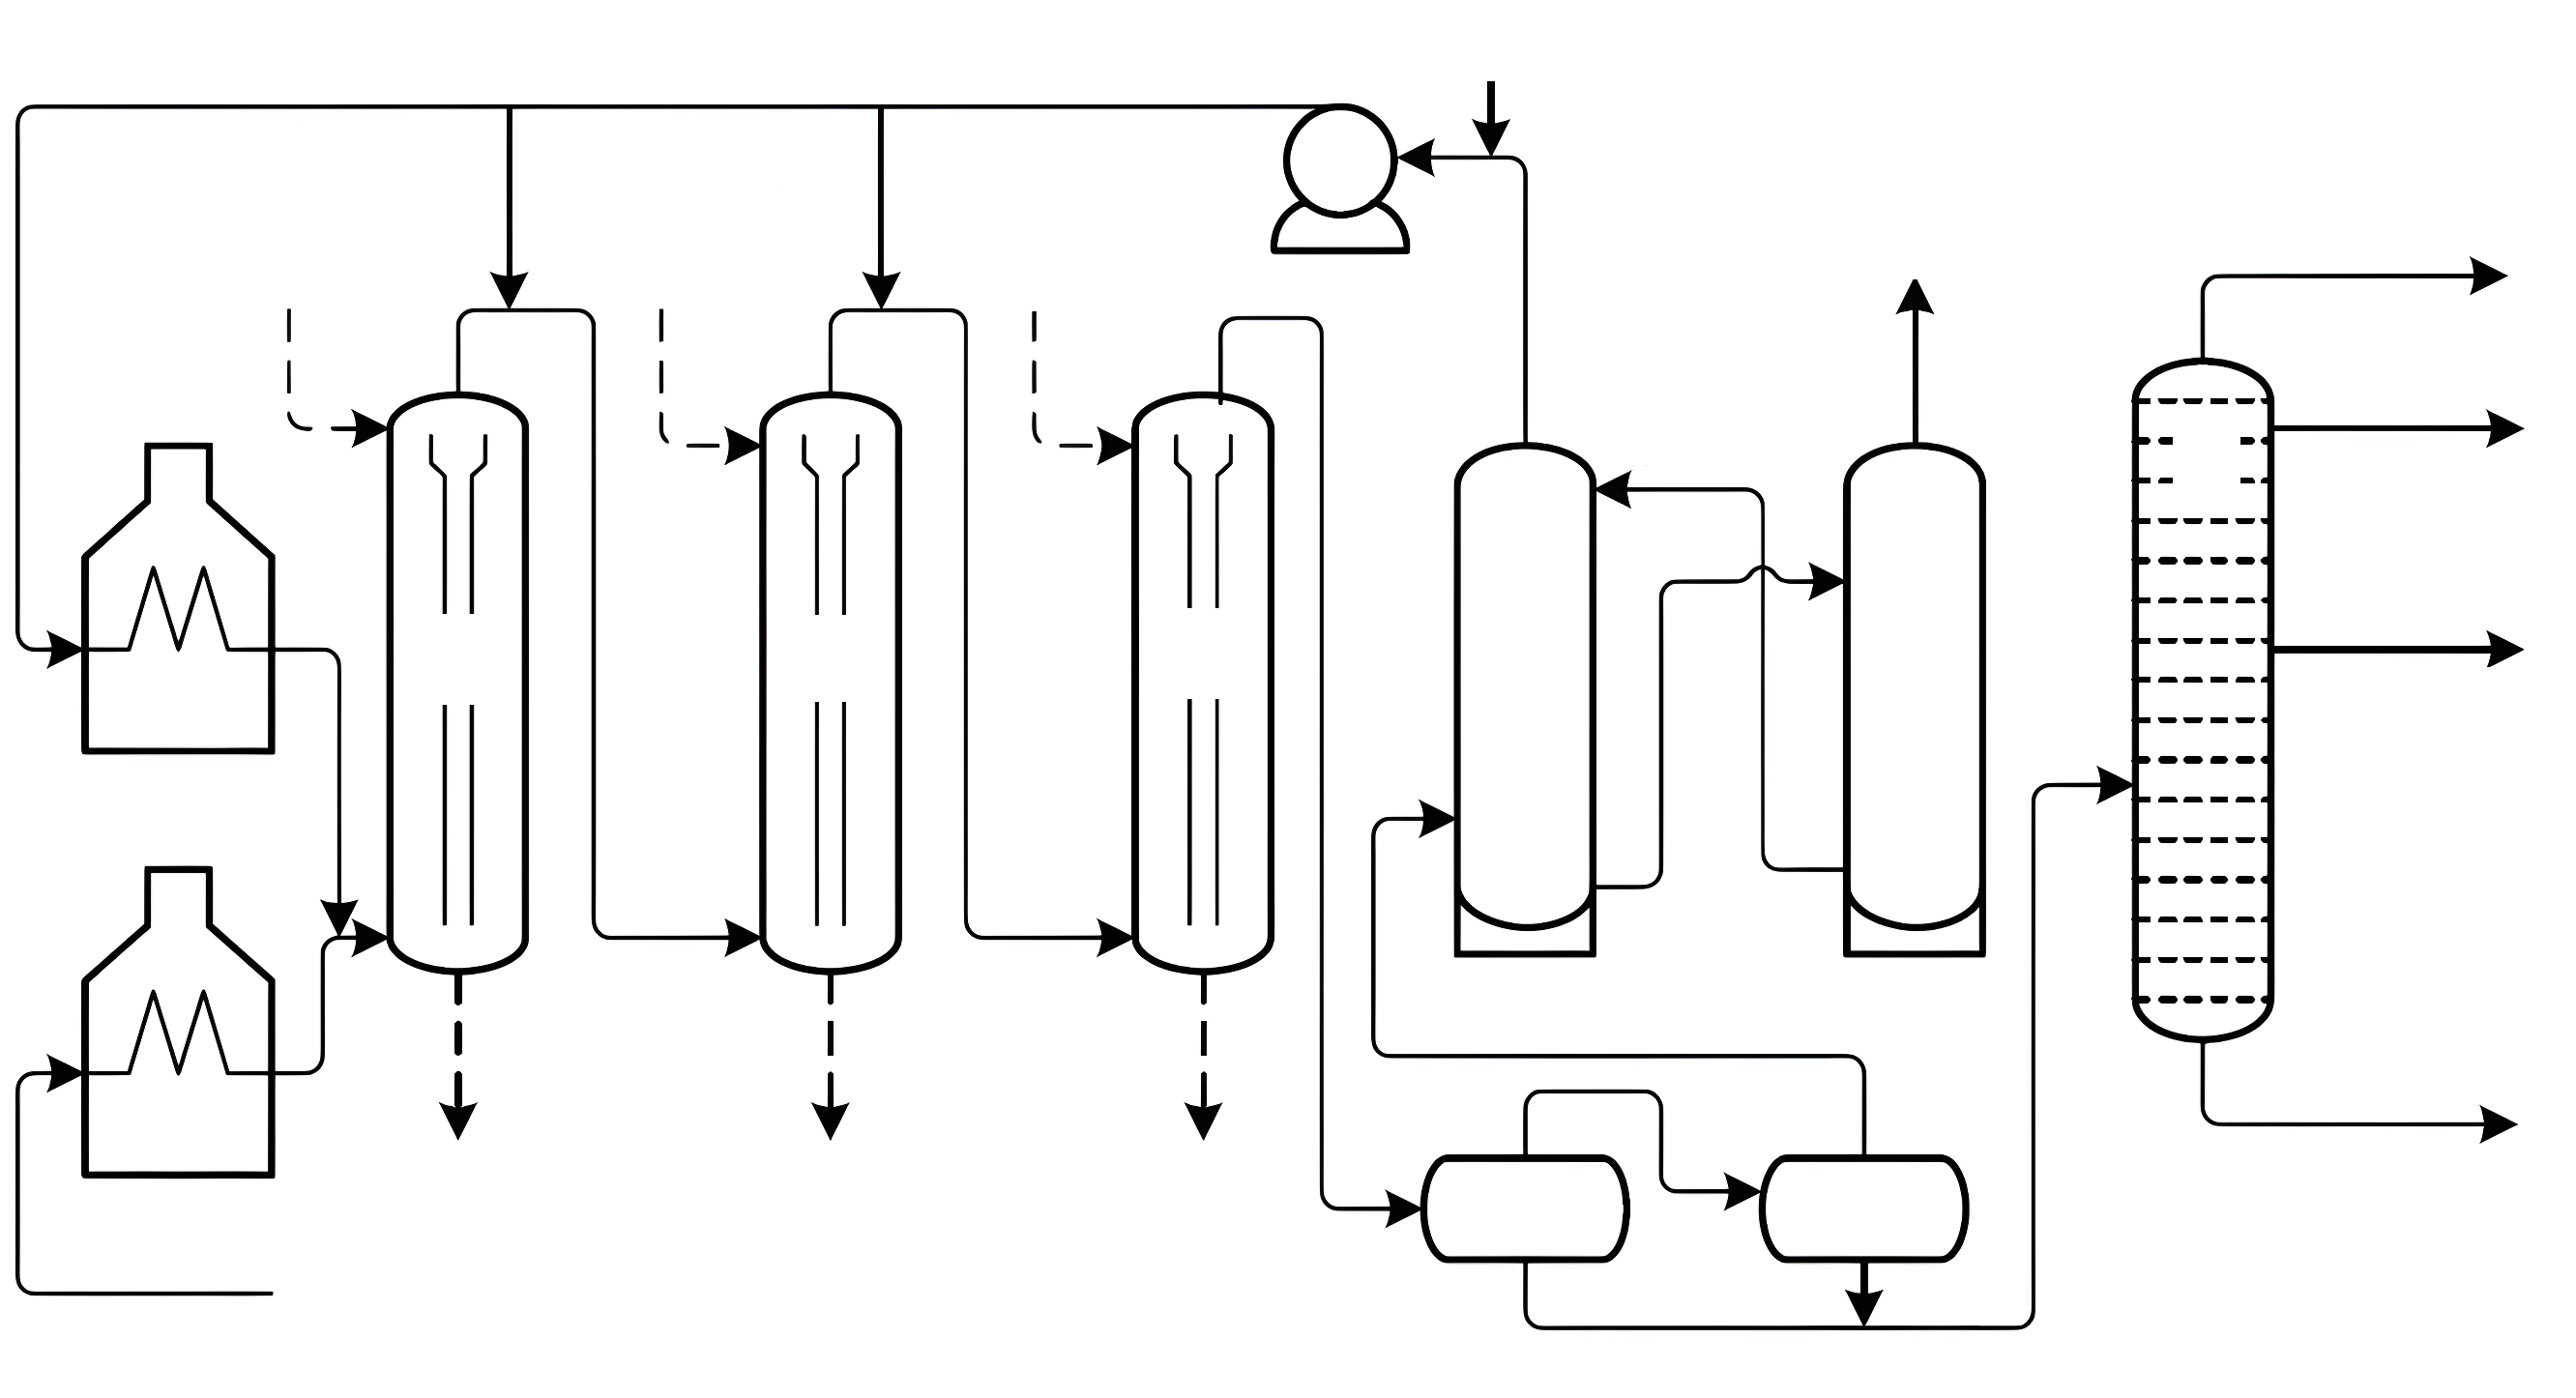
\includegraphics[width=0.8\textwidth]{figures/hydrokrak_Vschema.png}};
\node[font=\small\bfseries] at (-4.83,-1.85) {1};
\node[font=\small\bfseries] at (-4.83,0) {1};
\node[font=\small\bfseries] at (-3.6,0.2) {2};
\node[font=\small\bfseries] at (-2,0.2) {2};
\node[font=\small\bfseries] at (-0.37,0.2) {2};
\node[font=\small\bfseries] at (0.22,2.34) {3};
\node[font=\small\bfseries] at (1,-2.2) {4};
\node[font=\small\bfseries] at (2.5,-2.2) {5};
\node[font=\small\bfseries] at (3.983,1.03) {6};
\node[font=\small\bfseries] at (1.02,0.6) {7};
\node[font=\small\bfseries] at (2.72,0.6) {8};

\node[font=\small] at (-4.85,-2.8) {surovina};
\node[font=\small] at (-2.4,2.82) {recykl \ce{H2}};
\node[font=\small] at (2,1.22) {amin\footnotemark};
\node[font=\small] at (1.1,2.92) {čerstvý \ce{H2}};
\node[font=\small,align=center] at (2.72,2.3) {kyselé\\plyny};

\node[font=\small,align=center] at (-4.2,2.167) {nový\\kat.};
\node[font=\small,align=center] at (-2.6,2.167) {nový\\kat.};
\node[font=\small,align=center] at (-1,2.167) {nový\\kat.};
\node[font=\small,align=center] at (-3.6,-2.4) {deakt.\\kat.};
\node[font=\small,align=center] at (-2,-2.4) {deakt.\\kat.};
\node[font=\small,align=center] at (-0.4,-2.4) {deakt.\\kat.};

\node[font=\small] at (4.65,2.1) {plyny};
\node[font=\small] at (4.85,1.5) {benzin};
\node[font=\small,align=left] at (5,-0.35) {plynový\\olej};
\node[font=\small,align=center] at (4.55,-2.4) {nízkosirný\\těžký olej};

\end{tikzpicture}
    \caption[Schéma hydrokrakování frakcí v reaktorech s fluidním ložem]{Schéma hydrokrakování frakcí v reaktorech \textbf{s fluidním ložem} \cite{Blazek2006}.\\(1 - pec, 2 - hydrokrakovací reaktor, 3 - vodíkový kompresor, 4 - vysokotlaký separátor, 5 - nízkotlaký separátor, 6 - frakční kolona, 7 - absorbér vypírky plynů, 8 - desorbér) } \label{fig:hydrokrak_Vschema}
\end{figure}
\footnotetext{Aminy jsou chemické látky podobné amoniaku kde jsou jeden, dva nebo všechny tři atomy vodíku jsou nahrazeny organickými skupinami (např. alkyly \ce{C_nH_{2n+1}}). \cite{Boxer1997}}

\noindent
U varianty s fluidním ložem (Obr. \ref{fig:hydrokrak_Vschema}) je udržován konstantní běh hydrokrakovacích reaktorů souvislým nahrazováním deaktivovaných katalyzátoru katalyzátory novými za plného provozu. Hydrokrakovací jednotka funguje velmi podobně jako v konfiguraci s pevným ložem (Obr. \ref{fig:hydrokrak_Pschema}) s rozdílem toho, že nástřik suroviny společně s odvodem deaktivovaného katalyzátoru je prováděn spodem hydrokrakovacích reaktorů. Výhodou tohoto uspořádání je lepší kvalita a homogennost složení získaných produktů kvůli rovnoměrnému rozprostření katalytické směsi v reaktoru. \cite{Blazek2006,Prajapati2021}

\subsection{Odstranění nežádoucích složek z ropných frakcí}

V ropných frakcích, které se používají na výrobu pohonných hmot, je velmi často přítomna síra ve formě sirných sloučenin, především pak sulfidů. Při spalování pohonných hmot v komoře spalovacího motoru pak dochází k uvolňování síry ve formě oxidu siřičitého (\ce{SO2}), který je jako jedovatý plyn nebezpečný pro životní prostředí. Dalším nezanedbatelným negativem je vlastnost sirných sloučenin působit jako katalytický jed, jak už na katalyzátory používané při výrobě pohonných hmot, tak i na katalyzátory výfukových plynů automobilů. \cite{Blazek2006}
\begin{figure}[h]
    \centering
    \begin{tikzpicture}
\node[inner sep=0pt] (obrazek) at (0,0)
    {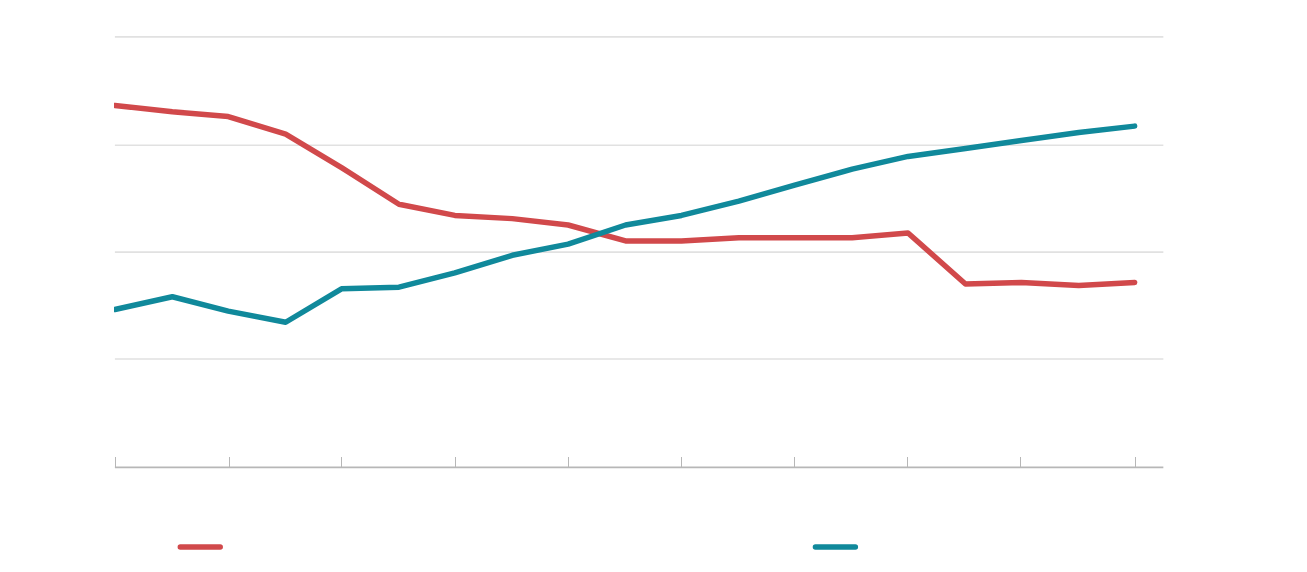
\includegraphics[width=0.9\textwidth]{figures/siravrope.png}};
\node[font=\small] at (-5,-2.05) {2005};
\node[font=\small] at (-4.07,-2.05) {2007};
\node[font=\small] at (-2.99,-2.05) {2009};
\node[font=\small] at (-1.9,-2.05) {2011};
\node[font=\small] at (-0.82,-2.05) {2013};
\node[font=\small] at (0.28,-2.05) {2015};
\node[font=\small] at (1.35,-2.05) {2017};
\node[font=\small] at (2.44,-2.05) {2019};
\node[font=\small] at (3.54,-2.05) {2021};
\node[font=\small] at (4.65,-2.05) {2023};

\node[font=\scriptsize] at (-1.7,-2.52) {Dovolené množství síry v produktech};
\node[font=\scriptsize] at (3.3,-2.52) {Poptávka po ropě};

\node[font=\small] at (-5.55,-1.76) {5};
\node[font=\small] at (-5.65,-0.72) {10};
\node[font=\small] at (-5.65,0.32) {15};
\node[font=\small] at (-5.65,1.34) {20};
\node[font=\small] at (-5.65,2.4) {25};

\node[font=\small] at (5.35,-1.76) {70};
\node[font=\small] at (5.35,-0.72) {80};
\node[font=\small] at (5.35,0.32) {90};
\node[font=\small] at (5.42,1.34) {100};
\node[font=\small] at (5.42,2.4) {110};

\node[font=\footnotesize,rotate=90] at (-6.25,0.25) {Dovolené množství síry $[\mathrm{Mt/rok}]$};
\node[font=\footnotesize,rotate=90] at (6.18,0.39) {Poptávka po ropě $[\mathrm{Mb/den}]$\footnotemark};

\end{tikzpicture}
    \caption[Dovolený obsah síry v ropných produktech]{Dovolený obsah síry v ropných produktech \cite{IEAfuture}.}
    \label{fig:siravrope}
\end{figure}
\footnotetext{Jednotka [$\mathrm{Mb/den}$] reprezentuje objem v milionech barelů za den. $1\ 000\ 000\ \mathrm{\text{barelů ropy}} = 158\ 987,3\ \mathrm{m^3} = 158\ 987\ 300 \ \mathrm{l}$.}

\noindent
Již od minulého století je vyvíjen tlak na výrobce pohonných hmot, aby vyráběné pohonné hmoty, ale i ropné produkty obecně, odsiřovaly v co největším míře. Rafinérie jsou v současné době schopny odstranit síru a sirné sloučeniny z ropných produktů až ze $70\%$. Trend zpracování ropy a poptávky po ropných produktech se bude v postupu let dále zvyšovat, kdežto dovolený obsah síry v produktech naopak rapidně klesá, viz. Obr. \ref{fig:siravrope}. \cite{IEAfuture} 

\subsubsection{Hydrogenační rafinace}
\label{subsubsec:hydrogenr}

Nejvyužívanější technologií rafinace ropných frakcí je katalytická hydrogenační rafinace. Používá se pro odstranění většiny nežádoucích sloučenin síry, dusíku a kyslíku z paliv. Kromě univerzálnosti je další výhodou schopnost dosáhnout vysokých výtěžků rafinátu, pohybujících se v intervalu $94\div99\ \mathrm{hm.}\%$ a nízké hustoty paliva. \cite{Blazek2006}

Produkty hydrogenační rafinace jsou bez přebytečných nenasycených molekul (např. olefínů), které by mohly ve větším množství způsobit oxidaci paliv. Takové palivo by mělo nižší cetanové číslo a tedy nižší tendenci ke vznícení. \cite{Seddon2022}

Schéma celého procesu hydrogenační rafinace frakcí s následujícím popisem procesů je znázorněno na Obr. \ref{fig:hydrogenr}.
\begin{figure}[h]
    \centering
    \begin{tikzpicture}
\node[inner sep=0pt] (obrazek) at (0,0)
    {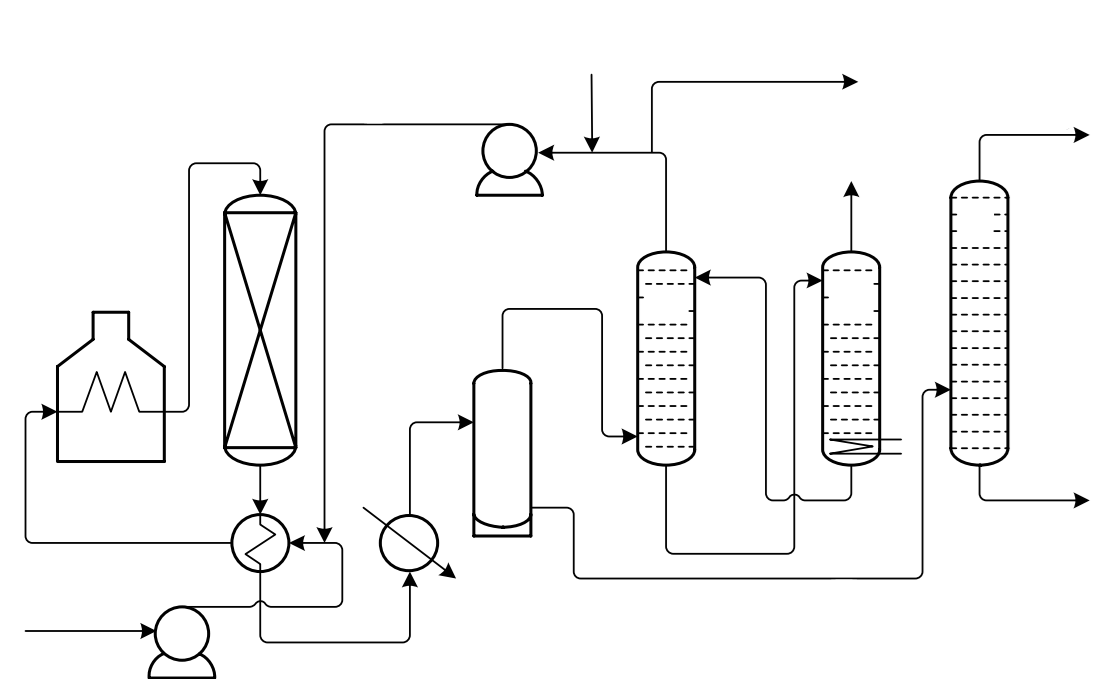
\includegraphics[width=0.8\textwidth]{figures/hydrogenr.png}};
\node[font=\small\bfseries] at (-3.75,-2.95) {1};
\node[font=\small\bfseries] at (-4.47,-0.885) {2};
\node[font=\small\bfseries] at (-2.95,1.1) {3};
\node[font=\small\bfseries] at (-0.475,-0.65) {4};
\node[font=\small\bfseries] at (1.2,0.4) {5};
\node[font=\small\bfseries] at (3.1,0.4) {6};
\node[font=\small\bfseries] at (4.4,1.25) {7};
\node[font=\small\bfseries] at (-0.4,2) {8};

\node[font=\small] at (-4.92,-3.15) {surovina};
\node[font=\scriptsize] at (-0.4,0.58) {vodíkový plyn};
\node[font=\scriptsize,align=center] at (-1.5,1.85) {cirkulační\\plyn};
\node[font=\scriptsize] at (0.45,2.96) {vodík};
\node[font=\scriptsize] at (2,2.96) {vodíkový plyn};
\node[font=\scriptsize] at (3.1,1.9) {sulfan};
\node[font=\scriptsize] at (1.9,-2.63) {kapalný produkt};
\node[font=\scriptsize,align=center] at (4.7,2.6) {\ce{C3} a \ce{C4}\\uhlovodíky};
\node[font=\scriptsize,align=center] at (4.8,-2.1) {odsířený\\produkt};
\end{tikzpicture}
    \caption[Schéma hydrogenační rafinace frakcí]{Schéma hydrogenační rafinace frakcí \cite{Blazek2006}.\\(1 - nástřikové čerpadlo, 2 - trubková pec, 3 - hydrorafinační reaktor, 4 - separátor vodíku, 5 - absorbér, 6 - regenerátor, 7 - frakční kolona, 8 - vodíkový kompresor)} \label{fig:hydrogenr}
\end{figure}

\noindent
V první části procesu rafinace se surovina (většina frakcí, které jsou produktem hydrokrakování) smíchá s vodíkem a v trubkové peci (\textbf{2}) se zahřívá ve směsi s dalšími reakčními produkty na obvyklé reakční parametry uvedené v následující Tab. \ref{tab:rp_hydrogenr}.
\begin{table}[h]
    \centering
    \begin{tabular}{|c|c|}
        \hline
        \textbf{Parametr reakce} & \textbf{Hodnoty a jednotky} \\ \hline\hline
        Teplota & $340\div420\ \mathrm{^{\circ}C}$ \\ \hline
        Tlak & $2 \div 6\ \mathrm{MPa}$ \\ \hline
        Poměr vodíku a suroviny & $200\ \mathrm{m^3_{suroviny}/m^3_{\ce{H2}}}$ \\ \hline
        Objemová rychlost & $5\ \mathrm{m^3_{suroviny}/h}$ na $1\ \mathrm{m^3_{\text{katalyzátoru}}}$ \\ \hline
        Spotřeba vodíku na odsíření & $0,8\ \mathrm{m^3_{\ce{H2}}/m^3_{suroviny}}$ \\ \hline
    \end{tabular}
    \caption[Reakční podmínky hydrogenační rafinace]{Reakční podmínky hydrogenační rafinace \cite{Seddon2022,Blazek2006}.}
    \label{tab:rp_hydrogenr}
\end{table}

\noindent
V další části směs putuje do hydrorafinačního reaktoru (\textbf{3)} a po následném ochlazení a snížení tlaku se v separátoru (\textbf{4}) uvolní vodíkový plyn. Tento plyn se dále vede do dvojice absorbéru a regenerátoru, kde se z něj vypírá sulfan a další kyselé oxidy síry. Část vodíkového plynu se recykluje a za přidání čerstvého vodíku putuje zpět do hydrorafinačního reaktoru. Nerecyklovaný vodíkový plyn se dá dále použít jako topný plyn v rafinérii nebo se z něj dá zpětně vyrobit čistý vodík způsoby uvedenými v následující kapitole práce. Již odsířené kapalné produkty se ze separátoru vedou do frakční kolony (\textbf{7}), kde produkt zbavuje přebytečných uhlovodíkových plynů. \cite{Blazek2006}

\subsubsection{Hydrogenační dearomatizace}

Dearomatizace je proces odstraňování aromatických uhlovodíků z ropných frakcí, především z benzinů a petrolejů. Aromatické uhlovodíky, přestože mají vysoké oktanové číslo a jsou tedy žádané v benzínech, jsou současně škodlivou složkou pro ovzduší kvůli jejich vysokým emisím uvolňujících se při spalování. V motorové naftě aromatické sloučeniny také zhoršují spalovací vlastnosti tím, že snižují cetanové číslo. Jejich přítomnost je tedy čistě nežádoucí. \cite{Blazek2006}

Aromatické uhlovodíky nelze odstranit běžnou destilací, protože mají body varu velmi blízké bodům varu jiných žádoucích uhlovodíků v dané frakci. K jejich odstranění se používají hydrogenační procesy, při kterých se aromatické uhlovodíky přeměňují na cykloalkany. Tento proces, označovaný jako hydrogenační dearomatizace, je vratnou exotermní reakcí, která se provádí při nízkých teplotách, aby se maximalizoval vznik cykloalkanů. \cite{Blazek2006}

Při použití dvoustupňové jednotky dearomatizace frakcí lze dosáhnout výsledků znázorněných v Tab. \ref{tab:dearomatizace}. Pří kombinaci této jednotky s jednotkou hydrogenační rafinace popsané v kapitole \ref{subsubsec:hydrogenr} lze dosáhnout i výrazného snížení obsahu síry a dusíku, popřípadě jejich oxidů a tím zvýšení cetanového čísla v tomto případě plynového oleje (produktu katalytického krakování). \cite{Blazek2006}
\begin{table}[h]
    \centering
    \begin{tabular}{|c|c|c|c|}
        \hline
        \thead{Parametr} & \thead{Surovina} & \thead{Produkt \\ z prvního \\ reaktoru} & \thead{Produkt \\ z druhého \\ reaktoru} \\ \hline\hline
        Hustota při $15\ \mathrm{^{\circ}C}$ [kg$\cdot$m$^{-3}$] & 942 & 873 & 856 \\ \hline
        Obsah \ce{S} [$\mathrm{mg_{\ce{S}}/kg_{produktu}}$] & $1,6\krat10^4$ & 3 & $< 0,5$ \\ \hline
        Obsah \ce{N} [$\mathrm{mg_{\ce{N}}/kg_{produktu}}$] & $1,1\krat10^4$ & 1 & $< 0,5$ \\ \hline
        Obsah aromátů $[\mathrm{hm.}\%]$ & 66 & 34 & 1,4 \\ \hline
        Cetanové číslo & 27 & 45 & 54 \\ \hline
    \end{tabular}
    \caption[Vlastnosti produktu dearomatizace plynového oleje z katalytického krakování]{Vlastnosti produktu dearomatizace plynového oleje z katalytického krakování \cite{Blazek2006}.}
    \label{tab:dearomatizace}
\end{table}